\chapter{Abschlussaufgabe Mean Shift}
Mean Shift ist ein parameterfreie Clusteralgorithmus bie welchem Punkte Clustern zugeordnet werden. Mean Shift findet Anwendung beim Clustering,
Tracking und bei Bildfiltern.\\
Nach einer Einführung in die Funktionsweise des Algorithmus wird eine sequentielle und parallele Implementation vorgestellt.
Abschließend werden Benchmarks zum Speedup und Laufzeit der Implementation betrachtet.\\
\begin{figure}[h]
	\centering
	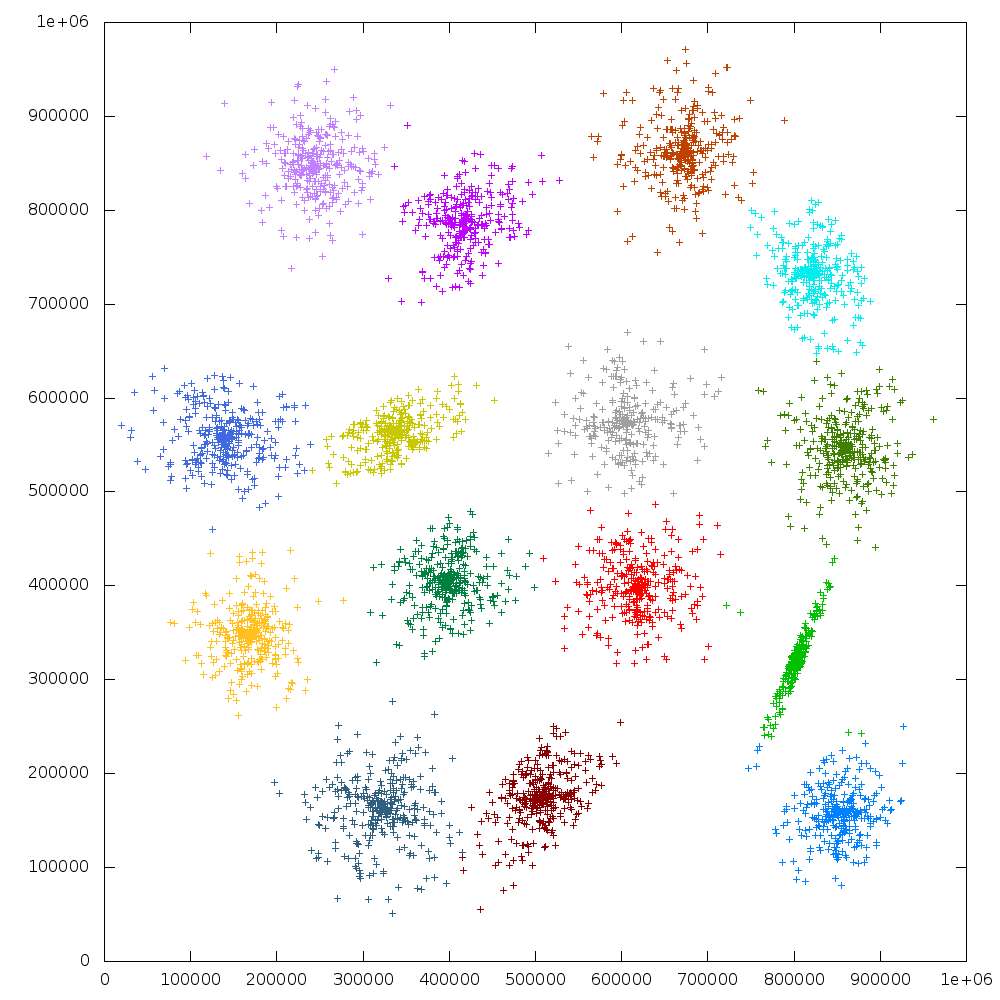
\includegraphics[scale=0.6]{../meanshift/output/pics/s1_colored.png} 
	\caption{Mean Shift S1.txt[B0]}
\end{figure}
\section{Algorithmus}
	Für jeden Punkt $ x $ der Eingabe wird ein Verschiebungsvektor $ m $ berechnet. 
		\[ m(x) = \frac{\sum_{x_i \in N(x)} K(x_i - x) x_i }{\sum_{x_i \in N(x)} K(x_i - x)} \]
	Die Punkte $ x_i $ werden in Abhängigkeit der Distanz zu $ x $ gewichtet. Hierfür wird in der Regel ein Gauß Filter eingesetzt.
		\[K(x_i - x) = e^{-c||x_i - x||^2} \]
	$ m(x) $ wird nun solange zu $ x $ addiert bis $ x $ konvergiert. Das Clusterzentrum von $ x $ ist genau der Grenzwert von $ x $.[1]\\
	Da für jeden Punkt unabhängig das Clusterzentrum bestimmt wird, lässt sich der Algorithmus durch Verteilung der zu berechnenden Punkte parallelisieren.\\
\section{Implementation}
	Mean Shift wurde in C implementiert. 
	Eingabe ist ein Menge von Koordinaten. Ausgabe ist eine Liste von Cluster Nummern. Die Visualisierung erfolgt mit Gnuplot.
	Dadurch wird der Code auf das Wesentliche beschränkt.
	Der sequentielle Algorithmus umfasst 100 LOC (Lines Of Code). Die Parallele MPI Version 170 LOC.\\
	Zur Wichtung wird ein 2D Gaußkern genutzt. Dieser muss normiert sein um ein oszillieren um ein Maximum zu verhindern.\\
	\vspace{-10pt}
	\begin{figure}[H]
		\centering
		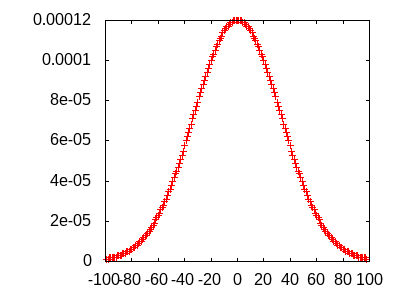
\includegraphics[scale=0.7]{../meanshift/output/pics/gauss.png} 
		\caption{Normierter Gaußkern S1.txt[B0]}
	\end{figure}
	Für die Testdaten[2] wurde experimentell eine passende Varianz bestimmt.\\
	Die Punkte werden in einer einfach verketteten Liste gespeichert. Durch speichern der Punkte in einer Baumstruktur welche den Ort der
	Punkte berücksichtigt lässt sich der Algorithmus optimieren. Weit entfernte Punkte können so ausgelassen werden.\\
	\subsection{MPI Parallelisierung}
	Beim MPI Mean Shift werden die zu berechnenden Punkte auf die Prozesse gleichverteilt.
	\lstset{language=C,
			basicstyle=\ttfamily,
			keywordstyle=\color{blue}\ttfamily,
			stringstyle=\color{red}\ttfamily,
			commentstyle=\color{green}\ttfamily,
			morecomment=[l][\color{magenta}]{\#}
	}
	\begin{lstlisting}
while(cur_point) {
    if(point_cntr % numprocs == rank)
        cur_point->cluster_nr = do_mean_shift(cur_point->x, cur_point->y);
    cur_point = cur_point->next;
    point_cntr++;
}
	\end{lstlisting}
	Anschließend werden die berechneten Cluster vom Hauptprozess (MPI Prozess mit Rank 0) wieder zusammengeführt und ausgegeben.\\
	Da die Punkte statisch den Rechenknoten zugewiesen werden ist eine vollständige Auslastung der Knoten nicht gewährleistet. 
	Dies könnte durch eine dynamische Verteilung der Punkte auf die Rechenknoten optimiert werden. Hier muss überprüft werden bei welchen Eingaben
	sich der höhere Verwaltungsaufwand lohnt.\\
	Durch Ungenauigkeiten der Fließkommazahlen konvergiert der Verschiebungsvektor $ m(x) $ nicht immmer. Daher muss ein geeignetes $ \delta $
	festgelegt werden. Bei Unterschreitung wird $ x $ als Clusterzentrum gespeichert. Bei Testdaten mit Punkten in einem 
	$ 1e + 06 $ großen Quadrat wurde $ \delta = 0.01 $ gewählt. Durch Vergrößern von $ \delta $ kann die Laufzeit des Algorithmus verringert werden.
	Die Anzahl der Fehlklassifikationen steigt jedoch mit $ \delta $ an.\\
	\vspace{-15pt}
	\begin{figure}[H]
		\centering
		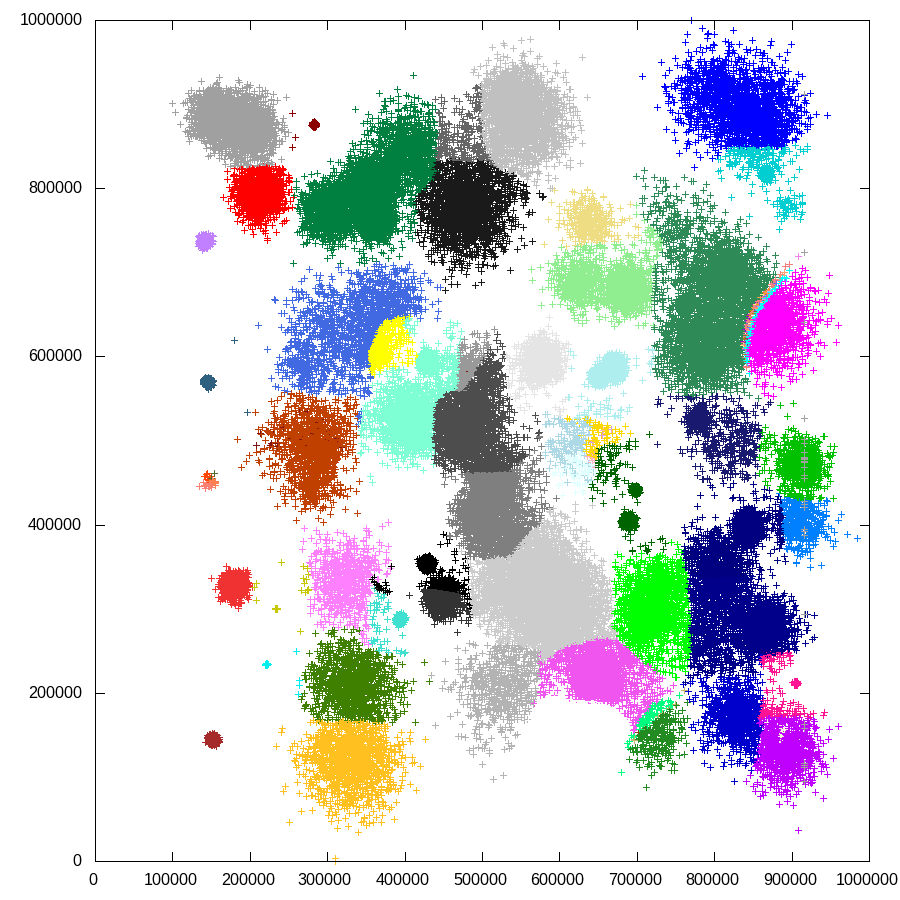
\includegraphics[scale=0.45]{../meanshift/output/pics/birch3_colored.png} 
		\vspace{-10pt}
		\caption{Birch3, 6 Minuten Laufzeit auf 128 Cores[B1]}
	\end{figure}
	\newpage
\section{Benchmark}
	Zum Benchmarking wurde die sequentielle und die MPI Version auf dem Hochleistungscluster Taurus[3] gemessen. Mit dem Batchsystem slurm wurden Datensätze mit
	5000 und 100000 Punkten auf 1, 2, 4, 8, 16, 32, 64, 128 und 256 Knoten gestartet. Die gemessene Laufzeit des MPI Jobs wird mit der sequentiellen
	Laufzeit verglichen.\\
	\begin{figure}[H] \centering
		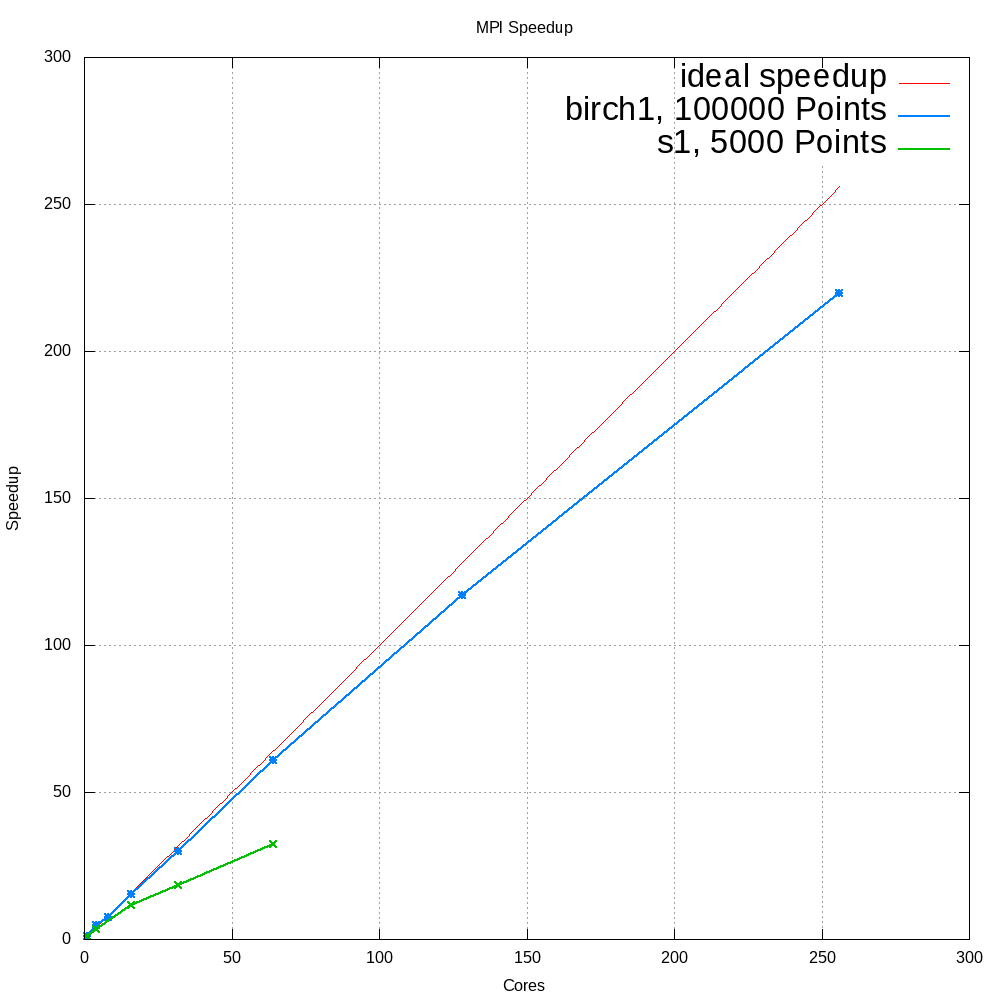
\includegraphics[scale=0.61]{../meanshift/output/pics/speedup.png} 
		\caption{Speedup [B1]}
	\end{figure}
	Bei steigender Anzahl an Cores nimmt der Speedup ab. Grund hierfür ist zum größten Teil die statische Verteilung der Punkte und die dadurch
	resultierende niedrigere Auslastung.\\
	\newpage
	\begin{figure}[H]
		\centering
		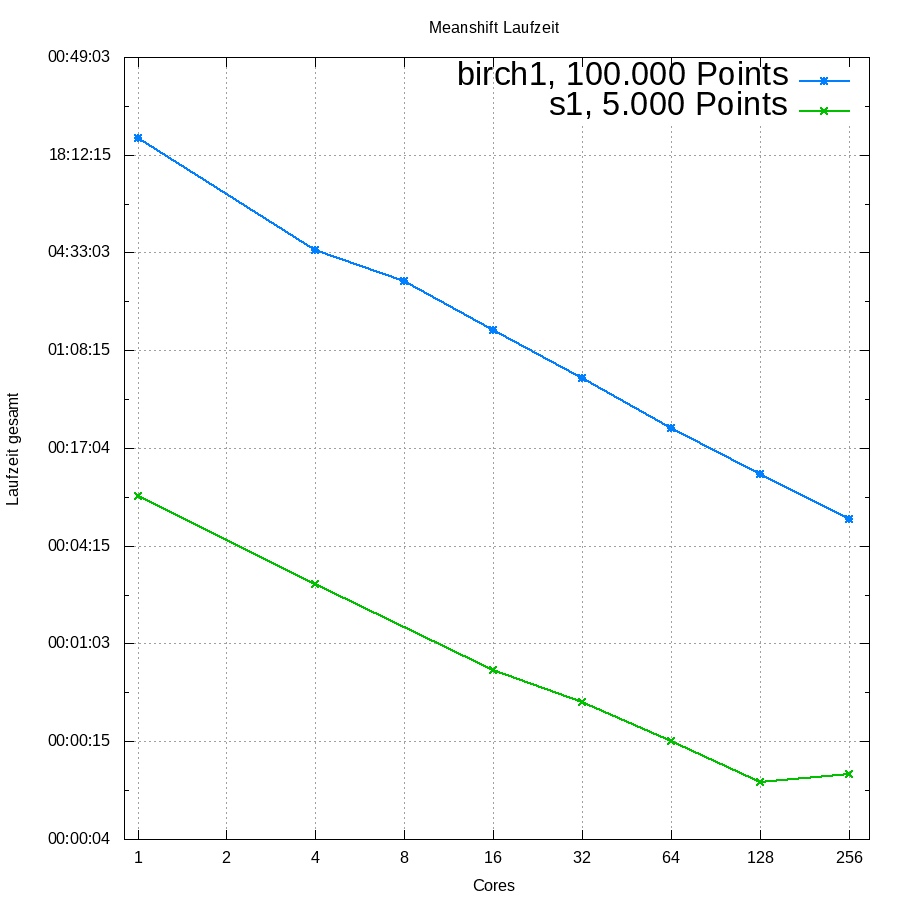
\includegraphics[scale=0.61]{../meanshift/output/pics/benchmark.png} 
		\caption{Laufzeit Benchmark[B1]}
	\end{figure}
	Bei 8 und  16 Cores zeigt sich eine Verschlechterung. Taurus hat jeweils zwei 8 Core CPUs auf einem Board.
	Ab 16 Cores läuft die Kommunikation über das Netzwerk.\\
	\newpage
\section{Fazit}
	Es existieren viele Möglichkeiten zur Optimierung des parallelen Algorithmus. Zum Beispiel eine dynamische Verteilung der Punkte oder eine dynamische Anpassung
	der Wichtung um die Anzahl der benötigten Mean Shifts zu verringern.\\
	Die Kernelgröße muss momentan noch manuell angegeben werden. Dies könnte auch automatisiert werden.\\
	\begin{figure}[H]
		\centering
		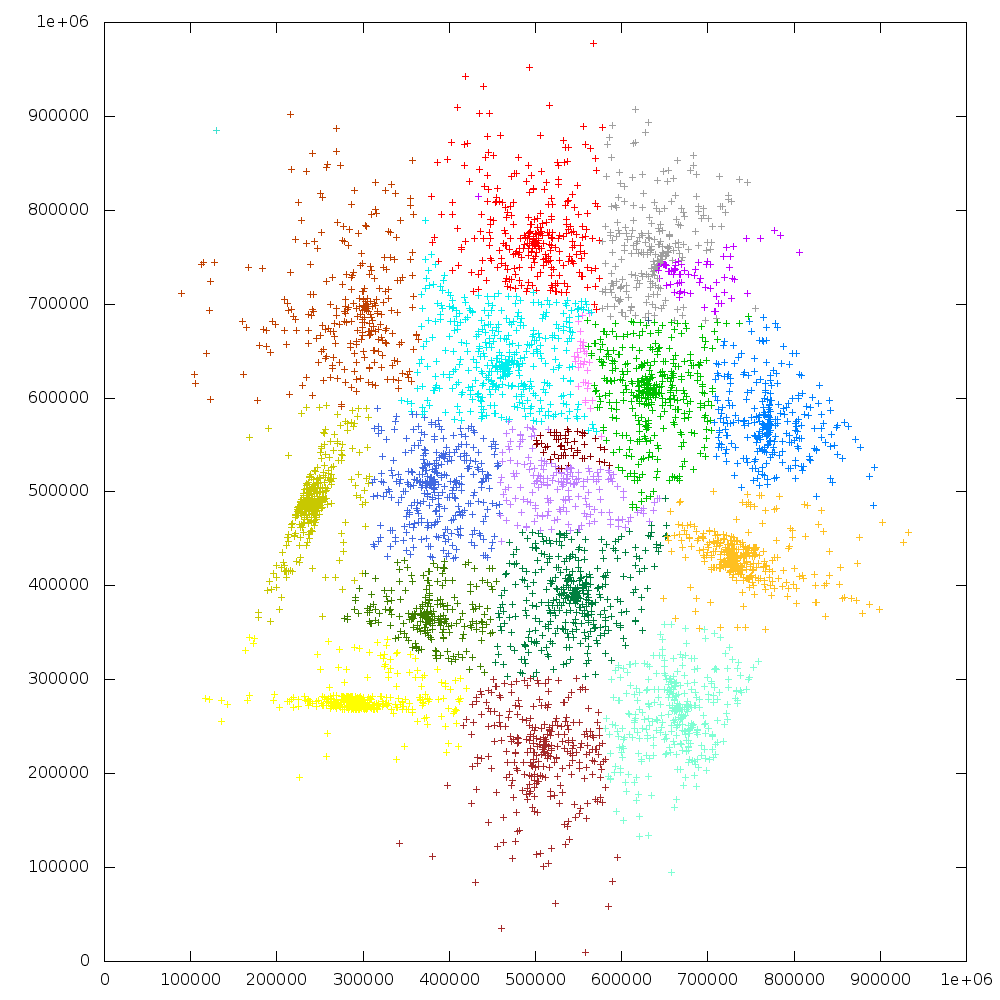
\includegraphics[scale=0.6]{../meanshift/output/pics/s4_colored.png} 
		\caption{S4, 5000 Points [B1]}
	\end{figure}
\begin{thebibliography}{999}
	\bibitem [0] {} Meanshift \url{http://homepages.inf.ed.ac.uk/rbf/CVonline/LOCAL_COPIES/TUZEL1/MeanShift.pdf}
	\bibitem [1] {} Mean Shift: Construction and Convergence Proof \url{http://www.cse.yorku.ca/~kosta/CompVis_Notes/mean_shift_derivation.pdf}
	\bibitem [2] {} Datasets \url{http://cs.joensuu.fi/sipu/datasets/}
	\bibitem [3] {} Taurus TU Dresden \url{https://doc.zih.tu-dresden.de/hpc-wiki/bin/view/Compendium/SystemTaurus}
	\bibitem [4] {} Meanshift \url{https://courses.csail.mit.edu/6.869/handouts/PAMIMeanshift.pdf}
	\newline
\end{thebibliography}
